% =====================================================================
%  Chapitre 6 -- Évaluation, interprétabilité et projet
%  Partie a : jeux de données, métriques, matrice de confusion, top-k
% =====================================================================
\section{Chapitre 6 --- Évaluation, interprétabilité et projet}

\chapterslide{Chapitre 6}{Évaluation, interprétabilité et projet}%
{5 h --- métriques, lecture des erreurs, visualisation, robustesse, projet GTSRB}%
{\textbf{Objectifs.} Choisir des jeux de données de référence et connaître leur coût ;
calculer et interpréter les métriques de classification (exactitude, précision, rappel, F1) ;
lire une matrice de confusion ; comprendre le top-$k$ et la courbe ROC ; visualiser ce
qu'un CNN a appris ; identifier ses limites ; mener le projet de classification de
panneaux routiers GTSRB.}

\begin{frame}{Plan du chapitre}
\begin{columns}[t]
\begin{column}{0.48\textwidth}
\begin{kbox}[Les quatre temps de ce chapitre]
\begin{enumerate}
  \item Les jeux de données de référence.
  \item Les métriques et leur lecture.
  \item L'interprétabilité : filtres, activations, Grad-CAM.
  \item Robustesse, limites et le projet GTSRB.
\end{enumerate}
\end{kbox}
\end{column}
\begin{column}{0.48\textwidth}
\begin{ebox}[Ce que vous saurez faire]
\begin{itemize}
  \item Choisir la métrique adaptée à une tâche.
  \item Diagnostiquer les erreurs d'un modèle avec une matrice de confusion.
  \item Visualiser et commenter ce qu'un CNN a retenu.
  \item Mener un projet de bout en bout, du jeu de données au rapport.
\end{itemize}
\end{ebox}
\end{column}
\end{columns}
\vspace{1mm}
\begin{wbox}[Un changement de regard]
Jusqu'ici, nous cherchions à \emph{construire} un réseau qui apprend. Ce chapitre
change de question : comment \textbf{savoir si ce qu'il a appris est juste}, et
\textbf{sur quoi il se trompe} ?
\end{wbox}
\end{frame}

\begin{frame}{Les jeux de données de référence}
\begin{center}
\footnotesize
\begin{tabular}{@{}llrl@{}}
\toprule
\textbf{Jeu de données} & \textbf{Contenu} & \textbf{Taille} & \textbf{Classes} \\
\midrule
MNIST & chiffres manuscrits $28\times28$, niveaux de gris & 70\,000 images & 10 \\
CIFAR-10 & photos couleur $32\times32$ (avion, chat, camion\dots) & 60\,000 images & 10 \\
ImageNet & photos couleur haute résolution, encyclopédique & $\approx$ 1,2\,M images & 1\,000 \\
\textbf{GTSRB} & \textbf{panneaux routiers réels, taille variable} & \textbf{39\,209 + 12\,630} & \textbf{43} \\
\bottomrule
\end{tabular}
\end{center}
\vspace{1mm}
\begin{columns}[t]
\begin{column}{0.48\textwidth}
\begin{itemize}
  \item La difficulté croît avec la variété : MNIST est « propre », GTSRB est \emph{réel}
  (éclairage, flou, cadrage variable).
  \item GTSRB sert d'échelle intermédiaire : assez petit pour un CPU,
  assez difficile pour être crédible.
\end{itemize}
\end{column}
\begin{column}{0.48\textwidth}
\begin{kbox}[Pourquoi ces jeux ?]
Ils sont tous \textbf{libres}, \textbf{documentés} et \textbf{comparables} : les résultats
publiés servent de repères. Un modèle évalué sur GTSRB se situe face à l'état de l'art.
\end{kbox}
\end{column}
\end{columns}
\end{frame}

\begin{frame}{GTSRB : le jeu du projet}
\begin{columns}[t]
\begin{column}{0.50\textwidth}
\centering
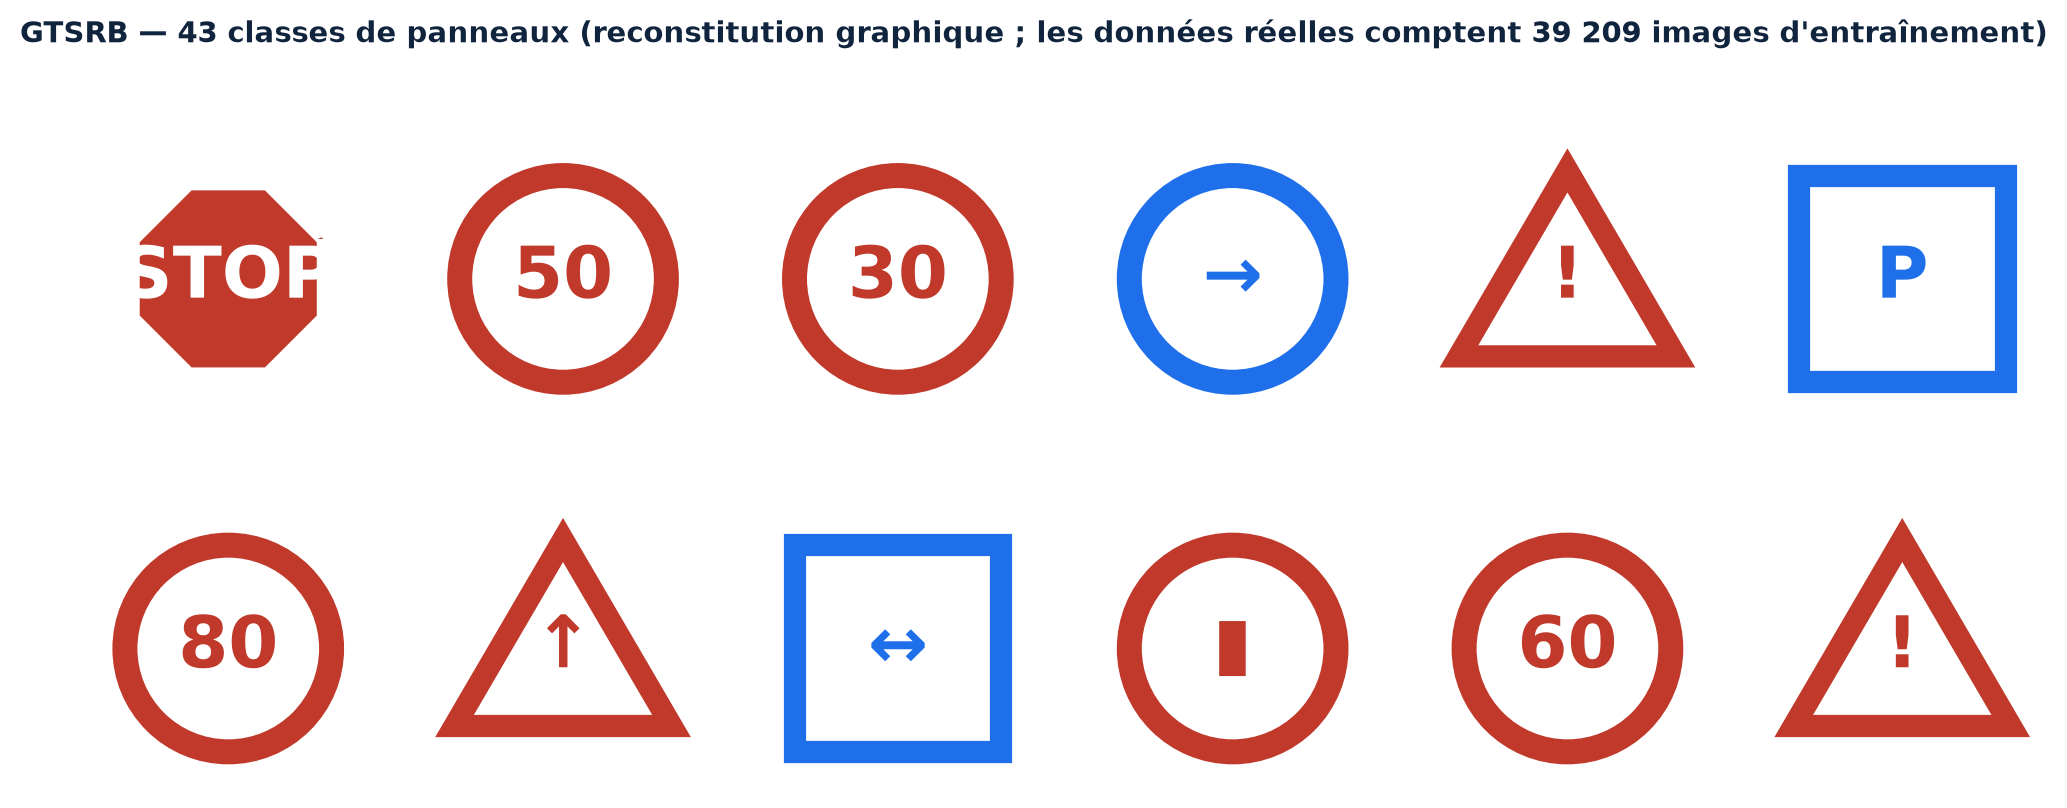
\includegraphics[width=0.48\textwidth]{k01_gtsrb.png}
\end{column}
\begin{column}{0.46\textwidth}
\begin{itemize}
  \item \textbf{39\,209} images d'entraînement.
  \item \textbf{12\,630} images de test.
  \item \textbf{43} classes (limitations, interdictions, obligations\dots).
  \item Tailles très variables : de \textbf{15 px} à \textbf{250 px} de côté.
\end{itemize}
\begin{wbox}[Le défi de GTSRB]
Les images n'ont pas toutes la même taille : il faut donc les
\textbf{redimensionner} (par exemple $32\times32$) ou adapter le réseau.
Le panneau peut être petit, flou, mal cadré.
\end{wbox}
\end{column}
\end{columns}
\end{frame}

\begin{frame}{Toujours trois sous-ensembles}
\begin{columns}[t]
\begin{column}{0.48\textwidth}
\begin{kbox}[Le découpage canonique]
\begin{itemize}
  \item \textbf{Entraînement} : le réseau apprend (\emph{train}).
  \item \textbf{Validation} : on règle les hyperparamètres (\emph{val}).
  \item \textbf{Test} : on mesure la performance finale, \emph{une seule fois}.
\end{itemize}
\end{kbox}
\end{column}
\begin{column}{0.48\textwidth}
\begin{wbox}[La fuite de données]
Si une image de test a servi à régler un paramètre, la performance mesurée
est \textbf{optimiste}. Le modèle a « vu » la réponse.
\end{wbox}
\begin{ebox}[Deux garde-fous]
\begin{itemize}
  \item Mélanger (\emph{shuffle}) avant de découper.
  \item Ne jamais toucher au jeu de test avant la fin.
\end{itemize}
\end{ebox}
\end{column}
\end{columns}
\end{frame}

\begin{frame}{Les quatre métriques de base}
\begin{columns}[t]
\begin{column}{0.48\textwidth}
\begin{itemize}
  \item \textbf{Exactitude} (\emph{accuracy}) : proportion de prédictions correctes.
  \[ \mathrm{Acc} = \frac{\text{prédictions correctes}}{\text{total}} \]
  \item \textbf{Précision} : parmi les objets annoncés « classe $c$ »,
  combien le sont vraiment ?
  \[ P_c = \frac{VP_c}{VP_c + FP_c} \]
\end{itemize}
\end{column}
\begin{column}{0.48\textwidth}
\begin{itemize}
  \item \textbf{Rappel} (\emph{recall}) : parmi les vrais objets de classe $c$,
  combien ont été trouvés ?
  \[ R_c = \frac{VP_c}{VP_c + FN_c} \]
  \item \textbf{F1} : moyenne harmonique de la précision et du rappel.
  \[ F1_c = 2\,\frac{P_c\,R_c}{P_c + R_c} \]
\end{itemize}
\end{column}
\end{columns}
\vspace{1mm}
\begin{kbox}[Vocabulaire]
$VP$ = vrai positif, $FP$ = faux positif (fausse alerte), $FN$ = faux négatif (oubli).
Le \textbf{F1} pénalise fortement un déséquilibre entre précision et rappel.
\end{kbox}
\end{frame}

\begin{frame}{La matrice de confusion}
\begin{columns}[t]
\begin{column}{0.56\textwidth}
\centering
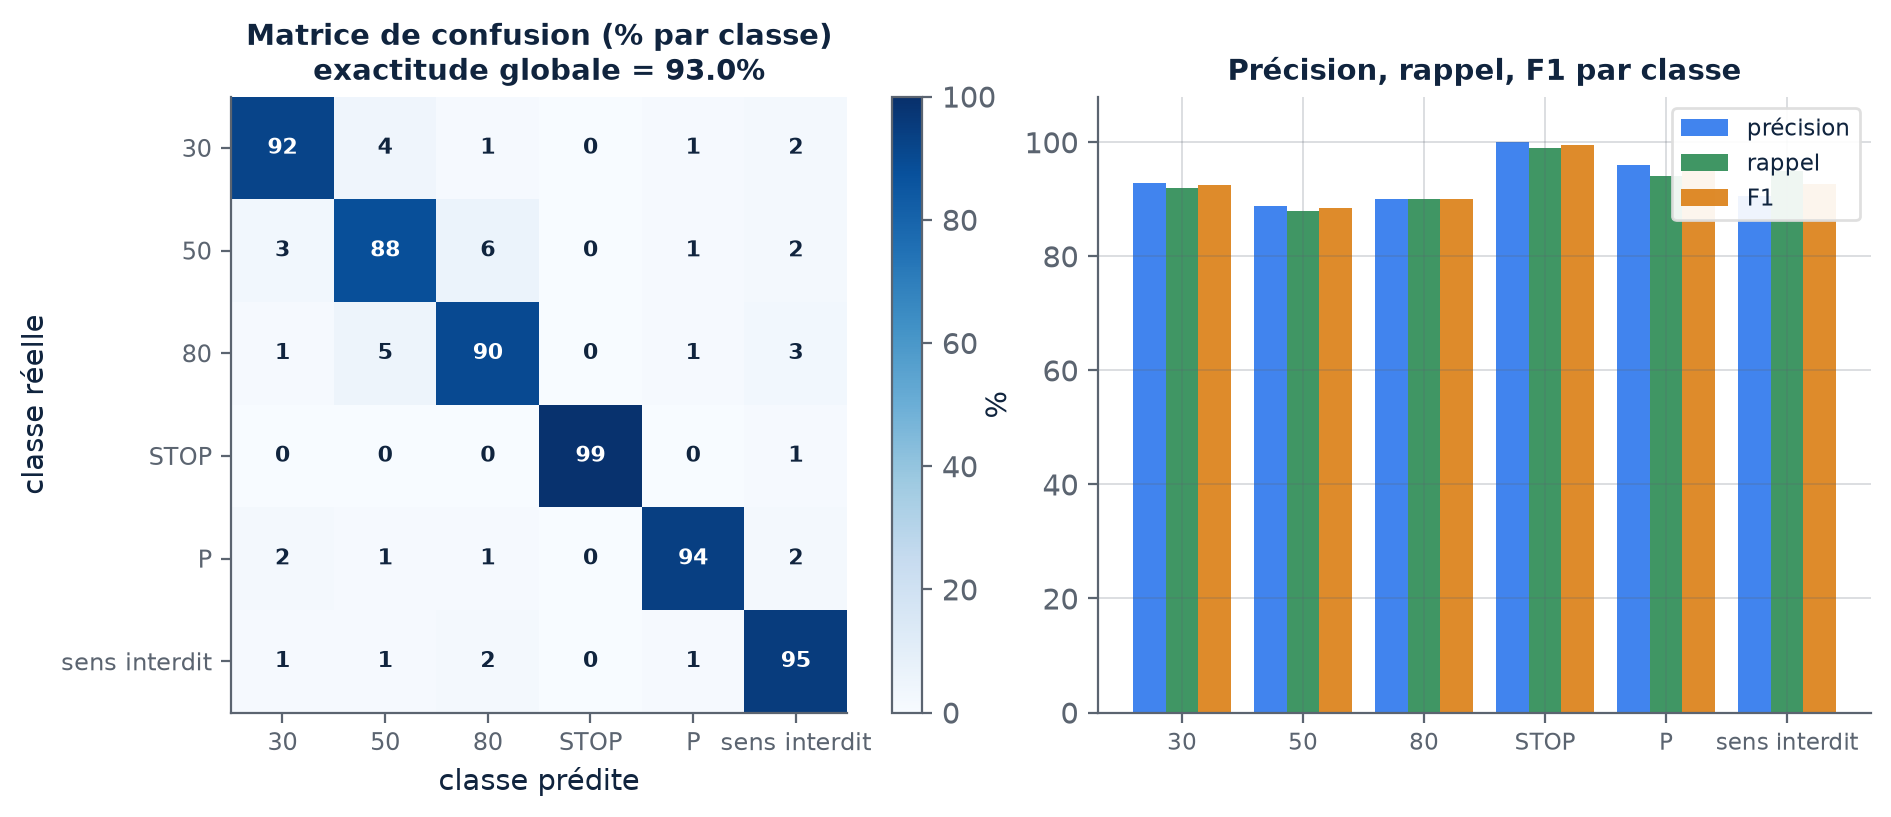
\includegraphics[width=0.54\textwidth]{k02_confusion_metriques.png}
\end{column}
\begin{column}{0.40\textwidth}
\begin{itemize}
  \item Ligne = classe \emph{réelle}, colonne = classe \emph{prédite}.
  \item La \textbf{diagonale} = les bonnes réponses.
  \item Hors diagonale = les \emph{confusions}.
  \item Exactitude mesurée sur ce sous-ensemble : \textbf{0,93}.
  \item F1 moyen : \textbf{0,9301}.
\end{itemize}
\begin{wbox}[La classe la plus faible]
La pire classe au sens du F1 est la classe \textbf{50} : c'est là qu'il faut
regarder en priorité pour progresser.
\end{wbox}
\end{column}
\end{columns}
\end{frame}

\begin{frame}[fragile]{Lire une matrice : un exemple chiffré}
\begin{columns}[t]
\begin{column}{0.50\textwidth}
\begin{center}
\scriptsize
\begin{tabular}{@{}l|rrrrrr@{}}
\toprule
& 30 & 50 & 80 & STOP & P & SI \\
\midrule
30    & 92 & 4 & 1 & 0 & 1 & 2 \\
50    & 3 & \textbf{88} & 6 & 0 & 1 & 2 \\
80    & 1 & 5 & 90 & 0 & 1 & 3 \\
STOP  & 0 & 0 & 0 & 99 & 0 & 1 \\
P     & 2 & 1 & 1 & 0 & 94 & 2 \\
SI    & 1 & 1 & 2 & 0 & 1 & 95 \\
\bottomrule
\end{tabular}
\end{center}
\vspace{1mm}
{\scriptsize Ligne $=$ vérité, colonne $=$ prédiction. \emph{SI} = sens interdit.}
\end{column}
\begin{column}{0.46\textwidth}
\begin{kbox}[Classe « 50 » : le calcul]
Sur 100 panneaux « 50 » réels :
\begin{itemize}
  \item $VP = 88$, $FN = 12$ $\Rightarrow$ rappel $= 0{,}88$.
  \item Sur 99 fois annoncés « 50 », 88 sont corrects
  $\Rightarrow$ précision $= 88/99 \approx 0{,}89$.
  \item $F1 \approx 0{,}88$ : la plus faible du tableau.
\end{itemize}
\end{kbox}
\begin{wbox}[Diagnostic]
6 panneaux « 50 » sont prédits « 80 », 5 « 80 » sont prédits « 50 » : ces deux
classes se \textbf{ressemblent} (chiffres blancs sur fond rouge). C'est une piste
d'amélioration concrète.
\end{wbox}
\end{column}
\end{columns}
\end{frame}

\begin{frame}[fragile]{Calculer ces chiffres avec scikit-learn}
\begin{columns}[t]
\begin{column}{0.53\textwidth}
\begin{codebox}[Matrice et rapport]
\begin{lstlisting}
from sklearn.metrics import confusion_matrix
from sklearn.metrics import classification_report

cm = confusion_matrix(y_vrai, y_pred)
print(cm)                  # matrice NxN

print(classification_report(
    y_vrai, y_pred,
    target_names=noms_classes))
# -> precision / recall / f1-score
#    par classe + moyenne
\end{lstlisting}
\end{codebox}
\end{column}
\begin{column}{0.43\textwidth}
\begin{itemize}
  \item On fournit la vérité (\file{y\_vrai}) et la prédiction (\file{y\_pred}).
  \item Le rapport affiche $P$, $R$, $F1$ \emph{par classe} : on repère
  immédiatement la classe faible.
  \item La \textbf{moyenne macro} traite chaque classe à égalité ;
  la \textbf{moyenne pondérée} tient compte de l'effectif.
\end{itemize}
\end{column}
\end{columns}
\end{frame}

\begin{frame}{Top-$k$ et courbe ROC}
\begin{columns}[t]
\begin{column}{0.52\textwidth}
\centering
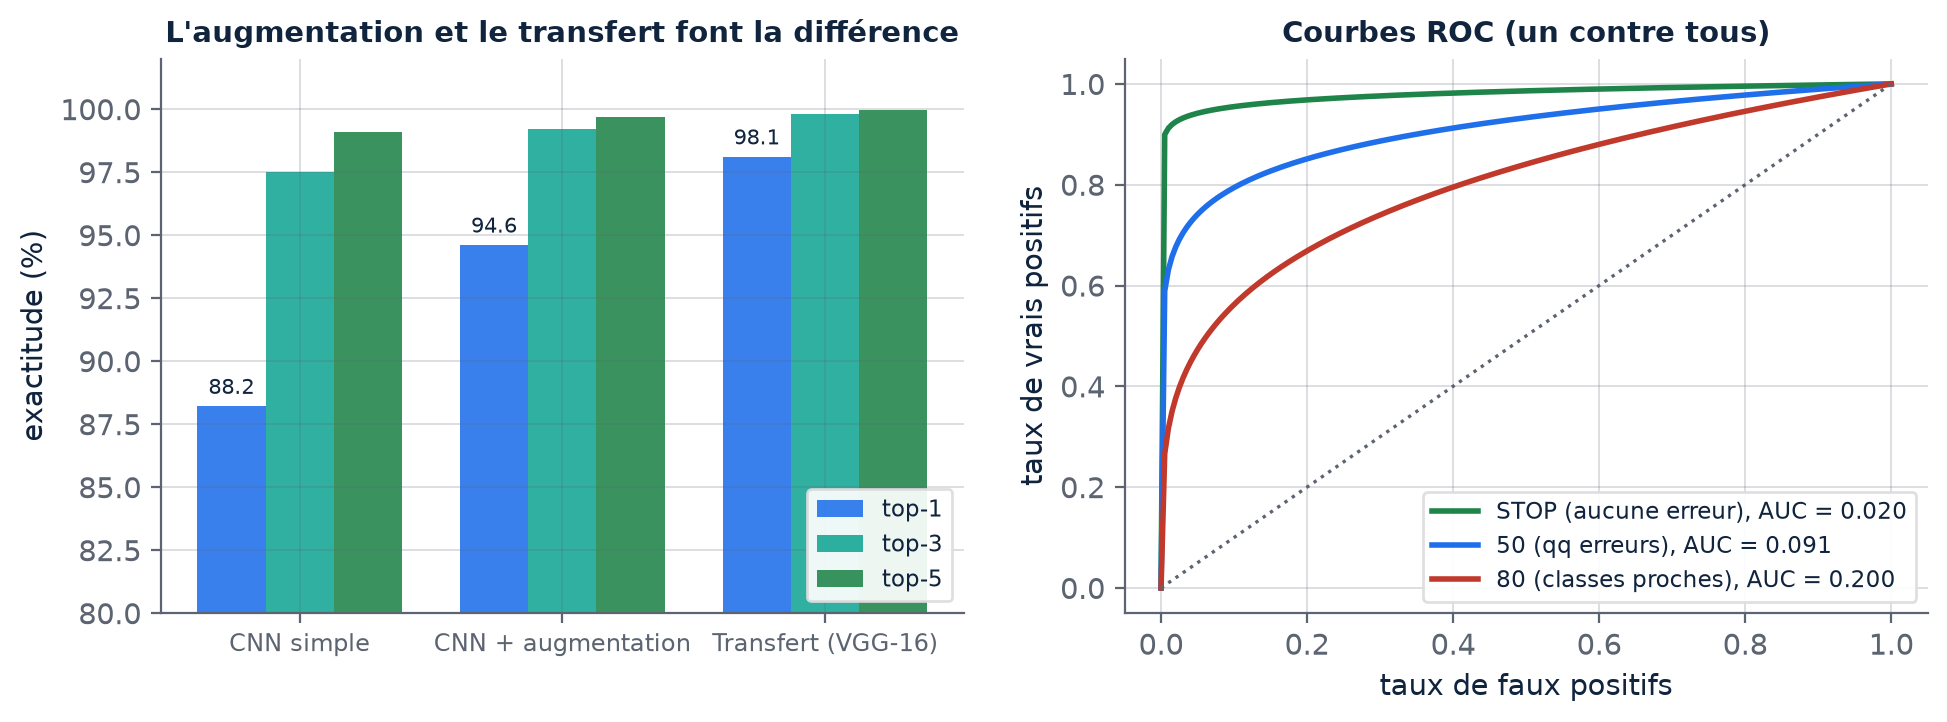
\includegraphics[width=0.50\textwidth]{k03_topk_roc.png}
\end{column}
\begin{column}{0.44\textwidth}
\begin{itemize}
  \item \textbf{Top-$k$} : le modèle donne ses $k$ meilleures classes ;
  on compte une réussite si la bonne classe y figure.
  \item Utile quand les erreurs « proches » sont acceptables.
  \item \textbf{Courbe ROC} : taux de vrais positifs en fonction du taux de
  faux positifs, en faisant varier le seuil.
  \item L'\textbf{AUC} (aire sous la courbe) résume la qualité : proche de 1
  = excellent, proche de 0,5 = hasard.
\end{itemize}
\end{column}
\end{columns}
\end{frame}

\begin{frame}{Top-$k$ : ce que la marge apporte}
\begin{columns}[t]
\begin{column}{0.50\textwidth}
\begin{center}
\footnotesize
\begin{tabular}{@{}lccc@{}}
\toprule
\textbf{Modèle} & \textbf{Top-1} & \textbf{Top-3} & \textbf{Top-5} \\
\midrule
CNN simple             & 88,2 & 97,5 & 99,1 \\
CNN + augmentation     & 94,6 & 99,2 & 99,7 \\
Transfert (VGG-16)     & 98,1 & 99,8 & 99,95 \\
\bottomrule
\end{tabular}
\end{center}
\end{column}
\begin{column}{0.46\textwidth}
\begin{itemize}
  \item Même le modèle simple retrouve la bonne classe dans ses 3 premières
  propositions \textbf{97,5 \%} du temps.
  \item Le top-1 progresse beaucoup plus vite que le top-5 : les modèles
  faibles « hésitent » sur de bons candidats.
  \item L'augmentation et le transfert apportent chacun un gain net.
\end{itemize}
\end{column}
\end{columns}
\end{frame}

\begin{frame}{Attention : l'exactitude seule trompe}
\begin{wbox}[Une métrique unique cache le pire]
Sur un jeu déséquilibré, un modèle peut afficher \textbf{93 \%} d'exactitude en
ignorant complètement une classe minoritaire. L'exactitude est la \emph{moyenne
de tout} : elle noie la classe rare.
\end{wbox}
\vspace{1mm}
\begin{columns}[t]
\begin{column}{0.48\textwidth}
\begin{kbox}[La bonne démarche]
\begin{itemize}
  \item Regarder $P$, $R$ et $F1$ \emph{classe par classe}.
  \item Identifier la pire classe et l'analyser.
  \item Choisir la métrique selon l'enjeu : en dépistage médical, on privilégie
  le \textbf{rappel}.
\end{itemize}
\end{kbox}
\end{column}
\begin{column}{0.48\textwidth}
\begin{ebox}[Exemple]
Si la classe « sens interdit » n'apparaît que 20 fois sur 1\,000 images, la rater à
chaque fois ne coûte que $2$ points d'exactitude\dots{} mais peut coûter très cher
sur la route.
\end{ebox}
\end{column}
\end{columns}
\end{frame}

\begin{frame}{À retenir --- première partie}
\begin{kbox}[Les idées clés de cette partie]
\begin{itemize}
  \item Trois jeux de référence : MNIST (chiffres), CIFAR-10 (photos), \textbf{GTSRB}
  (panneaux réels, 43 classes, de 15 à 250 px).
  \item Toujours découper en \textbf{entraînement / validation / test}, sans fuite.
  \item Quatre métriques : \textbf{exactitude}, \textbf{précision}, \textbf{rappel},
  \textbf{F1}.
  \item La \textbf{matrice de confusion} est l'outil de diagnostic : elle dit
  \emph{quelles} classes se confondent.
  \item Le \textbf{top-$k$} et la \textbf{courbe ROC / AUC} complètent le tableau.
  \item L'exactitude seule est trompeuse sur classes déséquilibrées.
\end{itemize}
\end{kbox}
\end{frame}
